\section{Cluster-based Map Abstraction}
\label{aha:mapabstraction}
The annotated graph we have focused on creating to now is sufficient for a low-level search but inefficient for large problem sizes. 
Instead of planning every step, we would prefer to express a more general strategy using macro-operators.
Our result from theorem {\ref{aha-theorem:reducibility} is key to the spatial abstraction described in this section. 
\par \indent
We extend the general process in \cite{botea04} which involves dividing a grid map into fixed-size square sections called \emph{clusters}. 
Adjacent pairs of clusters are connected to each other by \emph{entrances}, defined as obstacle-free transition areas of maximal size. 
Each entrance has one or two transition points (depending on its size) which are represented in the abstract graph by a pair of nodes connected with an undirected \emph{inter-edge} of weight 1.0. 
In Figure \ref{aha-fig:clustersandentrances}(a) we use clusters of size 5 to split our toy map into 4 adjacent sections. 
The highlighted region in Figure \ref{aha-fig:clustersandentrances} represents the maximally-sized entrance area between two clusters $\lbrace C1, C2 \rbrace$ while the connected tiles represent the transition point.
\begin{figure}[htbp]
        \caption{\emph{Building clusters and identifying entrances} }
        \begin{center}
                        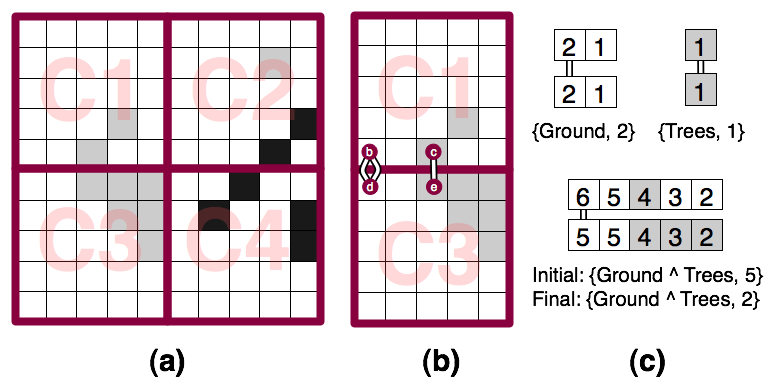
\includegraphics[scale=0.40]{diagrams/identifying_entrances.png}
        \end{center}
        \label{aha-fig:clustersandentrances}
\end{figure}
\par \indent
In the origial work each entrance area consists of a single line of tiles from each adjacent cluster and thus has an implicit \emph{depth}, $d = 1$.
This approach is adequate for small agents but unsuitable for larger agents as it produces incomplete abstract graphs. 
To demonstrate the validity of this claim, consider the example in Figure \ref{aha-fig:clustersandentrances}(c). 
Here we show a large agent $A$ of size 2 that begins in the same cluster as the goal location. 
Notice that there exists a valid solution to this problem as shown. 
Notice further however that in order for $A$ to reach the goal it cannot use the centre transition point as the associated clearance values are too small.
By limiting depth to $d = 1$ the entrance-building technique fails to detect the bottleneck region and means that not all valid paths in the low-level graph are found in the abstract graph.
To address this problem we consider a larger set of tiles; up to $d \leq max(s) \in S$  inside each cluster.
\par \indent
Starting at the pair of tiles at the beginning of each adjacent area we first extend the entrance symmetrically inside each cluster up to $d \leq max(s) \in S$ or until an obstacle is encountered for some capability $c \in C$.
We then extend the entrance's \emph{size} in an orthogonal direction, along the common border, computing depth at each step and continuing until one of three termination conditions occurs: the end of the adjacent area is reached, an obstacle is discovered or $d$ begins to increase or decrease in either cluster. 
The latter is important for detecting bottleneck regions such as those in Figure \ref{aha-fig:clustersandentrances}(c).
\par \indent
Once an entrance is found, we choose as the transition point the first pair of adjacent nodes in each cluster which maximise clearance for $c$.
This latter metric, $cv_{entrance}$ is computed by taking the minimum clearance among each pair of adjacent nodes in the entrance area and selecting the largest value from the set. 
Thus, we add a new edge to the graph, $e_{inter}$ and annotate it with a single capability and corresponding clearance value, $e_{inter}(c) = cv_{entrance}$. 
The algorithm repeats $\forall c \in C$ and terminates when all adjacent clusters have been considered. 
This ensures we identify all possible entrances for each available capability.
\par \indent
In figure \ref{aha-fig:clustersandentrances}(d) we present three entrances identified by scanning the border between clusters $C1$ and $C2$.
Entrances \emph{E1} and \emph{E3}, both of depth 2, are found at the beginning and end of the adjacent area; before and after the bottleneck region. 
Each resultant inter-edge is thus annotated as $\lbrace Ground, 2 \rbrace$ corresponding to the capability and maximal clearance of the entrance area.
\emph{E2} is a smaller entrance identified due to the change in depth, from 2 to 1. 
It also has smaller maximal clearance so its inter-edge is thus annotated as $\lbrace Ground, 1 \rbrace$.
In some scenarios the same location may correspond to a maximally sized transition point for several capabilities. 
To keep the size of the abstract graph small we actively attempt to re-use existing nodes and thus allow multiple edges between the same nodes.  
\par \indent
The final step in the decomposition involves attempting to add to the abstract graph a set of \emph{intra-edges} for each pair of abstract nodes inside a cluster. 
We achieve this by running multiple AA* searches $\forall (c, s) : c \in C, s \in S$.
Once a path is found we annotate the new edge, $e_{intra}$, with the capability and clearance parameters used by AA* and set its weight equal to the cost of the path. 
The algorithm terminates when all clusters have been considered. 
\par \indent
We thus construct an abstract \emph{multi-graph} in which each edge $e$ is annotated with a single capability $c_{e}$ and associated clearance value $cv_{e}$. These represent the minimum capability set that an agent $a$ must posess to traverse the edge, $c_{a}$, and the agent's maximum size, $s_{a}$. More succinctly:
$$ e(c_{a}) = cv_{e} \geq s_{a} : c_{e} \in c_{a} \in C$$
We term the resultant abstraction $initial$ and give the following lemmas to characterise its space complexity:

\input abstractionproperties
